\newcommand{\inhometopology}[0]{
\begin{tikzpicture}
[
    scale=0.6, 
    transform shape
    ] 
\sizearrowleft{(0,0)}{(0,8.85)}{8.85 meter};
\sizearrowbelow{(0,0)}{(8.85,0)}{8.85 meter};

\draw [fill=room backg](0,0) rectangle (4.42274,4.42274);
\draw [fill=room backg](0,4.42274) rectangle (4.42274,8.84549);
\draw [fill=room backg](4.42274,0) rectangle (8.84549,4.42274);
\draw[color=el cable, line width=2pt] (0.490256,0.416898) -- (0.490256,0.416898);
\draw[color=el cable, line width=2pt] (0.58487,0) -- (0.490256,0.416898);
\draw[color=el cable, line width=2pt] (0,1.24412) -- (0.490256,0.416898);
\draw[color=el cable, line width=2pt] (0.713926,4.97535) -- (0.490256,0.416898);
\draw[color=el cable, line width=2pt] (4.42274,5.31765) -- (0.713926,4.97535);
\draw[color=el cable, line width=2pt] (0,4.86111) -- (4.42274,5.31765);
\draw[color=el cable, line width=2pt] (5.14141,0.651136) -- (0.490256,0.416898);
\draw[color=el cable, line width=2pt] (4.55818,0) -- (5.14141,0.651136);
\draw[color=el cable, line width=2pt] (5.01992,4.42274) -- (5.14141,0.651136);
\node[inner sep=0pt] (n0) at (0.490256,0.416898) {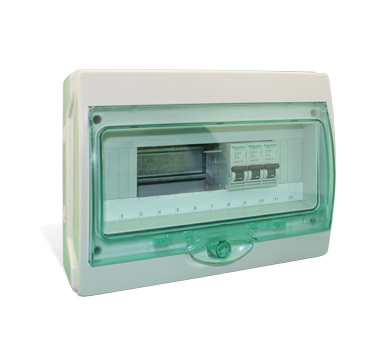
\includegraphics[width=.09\textwidth]{dist_box.png}};
\node[inner sep=0pt] (n1) at (0.58487,0) {
\includegraphics[width=.09\textwidth]{modem.png}};
\node[inner sep=0pt] (n2) at (0,1.24412) {
\includegraphics[width=.09\textwidth]{modem.png}};
\node[inner sep=0pt] (n7) at (0.713926,4.97535) {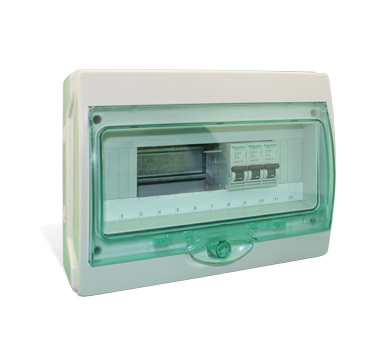
\includegraphics[width=.09\textwidth]{dist_box.png}};
\node[inner sep=0pt] (n3) at (4.42274,5.31765) {
\includegraphics[width=.09\textwidth]{el_dev.png}};
\node[inner sep=0pt] (n4) at (0,4.86111) {
\includegraphics[width=.09\textwidth]{modem.png}};
\node[inner sep=0pt] (n8) at (5.14141,0.651136) {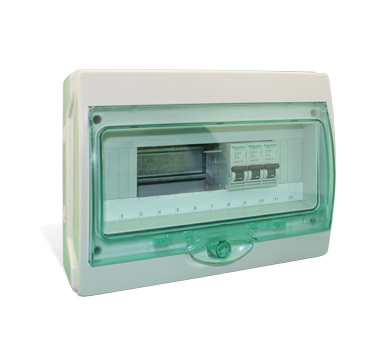
\includegraphics[width=.09\textwidth]{dist_box.png}};
\node[inner sep=0pt] (n5) at (4.55818,0) {
\includegraphics[width=.09\textwidth]{el_dev.png}};
\node[inner sep=0pt] (n6) at (5.01992,4.42274) {
\includegraphics[width=.09\textwidth]{el_dev.png}};
\end{tikzpicture}
}
